\documentclass[utf8,handout]{beamer}

\usepackage{presentation}
\title{Сервис поиска электронных книг}
\subtitle{Серверная часть, обеспечивающая хранение информации о~книгах, поиск по ней и возможность модифицировать её}

\author{Иваницкий Андрей}

\institute{Санкт-Петербургский Академический Университет РАН}
\date{\today}

\begin{document}

\begin{frame}
	\titlepage
\end{frame}

\section*{План презентации}
	\begin{frame}
		\frametitle{План презентации}
		\tableofcontents[pausesections]
	\end{frame}

\section{Описание внутренней структуры системы}
	\begin{frame}
		\frametitle{Описание внутренней структуры системы}
		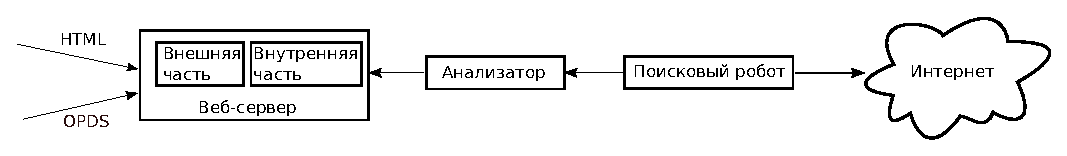
\includegraphics[width=1.05\textwidth]{./head/innerstructure}
	\end{frame}


\section{Постановка задачи}
	\begin{frame}
		\frametitle{Постановка задачи}
		\begin{block}{Поиск по данным}
			Мощный, быстрый и удобный поиск\\
			как для пользователя,\\
			так и для анализатора.
		\end{block}
		\begin{block}{Интерфейс модификации данных}
			Полный, гибкий и расширяемый интерфейс модификации данных для анализатора.
		\end{block}
	\end{frame}


\section{Поиск по данным}
	\begin{frame}
 		\frametitle{Поиск по данным}
 		\begin{block}{}
			Предоставляет
			\begin{enumerate}
				\item  Релевантный поиск как по отдельным сущностям, так и по различным их комбинациям;
				\item  Фильтрация результатов поиска по некоторым сущностям (язык книги, тэг);
				\item  Поиск с учётом морфологии языка;
				\item  Поиск среди авторов по звучанию;
				\item  Исправление опечаток в запросе;
				\item  Простой поиск (простой в использовании).
			\end{enumerate}
		\end{block}
	\end{frame}
	

\section{Интерфейс модификации данных}
	\subsection{Алгоритм взаимодействия с анализатором}
	\begin{frame}
 		\frametitle{Алгоритм взаимодействия с анализатором}
	\end{frame}
	
	\subsection{Фаза распознования}
	\begin{frame}
 		\frametitle{Фаза распознования}
 	\end{frame}

	\subsection{Расчёт расстояния между строками}
	\begin{frame}
 		\begin{block}{Алгоритм: \textbf{Расчёт расстояния между строками}}
 			Две строки $s_{1}$ и $s_{2}$ разбиваются на слова:
 			$s_{1}\rightarrow S_{1}=\lbrace a_{1},\ldots,a_{n}\rbrace$, $s_{2}\rightarrow S_{2}=\lbrace b_{2},\ldots,b_{m}\rbrace$ \\
 			Пусть $n\leq m$

			$ M_{i,j} = D_{Levenshtein}(a_{i},b_{j}), i=1..n, j=1..m $ \\
			где $D_{Levenshtein}$ --- расстояние Левенштейна
			
			\[	C_{min}=\min_{\alpha_1, \alpha_2, \ldots, \alpha_m}{\sum_{i=1}^{n} M_{i,\alpha_{i}}} \] \\
			где $\alpha_1, \alpha_2, \ldots, \alpha_m$ --- перестановка чисел от $1$ до $m$,\\
			минимум по всем таким возможным перестановкам

			$C_{full}=C_{min}+(m-n)\times C_{remove}$\\
			где $C_{remove}$ --- цена добавления/удаления слова.
		\end{block}
	\end{frame}

	\subsection{Фаза добавления}
		\begin{frame}[fragile]
 			\frametitle{Структура запроса}
 			\begin{verbatim}
<?xml version="1.0" encoding="UTF-8"?>
<request>
    <define>
        ...
    </define>

    <update>
        ...
    </update>
</request>
			\end{verbatim}
		\end{frame}
	
		\begin{frame}
 			\frametitle{Секция define}
		\end{frame}
	
		\begin{frame}
 			\frametitle{Секция update}
		\end{frame}
	
\section{Заключение}
	\begin{frame}
		\frametitle{Заключение}
	\end{frame}
	




\end{document}
